%定義

\documentclass[10pt,twocolumn]{jarticle} 
\usepackage{algorithm2e}
\usepackage{fancybox}
%\usepackage{here}
\usepackage[dvipdfmx]{graphicx}
%\usepackage[dvipdfmx]{hyperref}
\usepackage{comment}
\usepackage{amsmath}
\usepackage{amssymb}
\usepackage{amsthm}
\usepackage{amsfonts}
\usepackage{titlesec}
\usepackage{latexsym}
\usepackage{euler}
\usepackage{float}


\pagestyle{empty}

%余白とか

\setlength{\topmargin}{-3.0cm} 
\setlength{\textheight}{28.0cm} 
\setlength{\textwidth}{18.5cm}
\setlength{\oddsidemargin}{-1.3cm} 
\setlength{\columnsep}{.5cm}
\newcommand{\noin}{\noindent}
\catcode`@=\active \def@{\hspace{0.9bp}-\hspace{0.9bp}}
\newtheorem{dfn}{定義}[section]
\newtheorem{theorem}{定理}[section]


\makeatletter
\renewcommand{\section}{\@startsection{section}{1}{\z@}%
{1.5\Cvs \@plus.5\Cvs \@minus.2\Cvs}%
{.5\Cvs \@plus.3\Cvs}%
{\reset@font\Large\mcfamily}}
\makeatother

\renewcommand{\baselinestretch}{0.94}


%タイトル

\title{NFV上の最適経路割り当て問題}
\setcounter{footnote}{1}
\author{田中研究室:河本　明日翔\if0\thanks{神奈川大学理学部情報科学科 田中研究室}\fi}
\date{\today}

%タイトル作成

\begin{document}

\maketitle
\thispagestyle{empty}


\section{はじめに}
\noindent　仮想ネットワーク埋め込み問題
（Virtual Network Embedding Problem：VNE）とは，
仮想ノードと仮想リンクから構成されるVN要求を，
物理ネットワーク上の物理ノードと物理リンクへ割り当てる問題である．
VNEはNP困難であるため，実用的な時間で解を求める発見的解法が研究されている\cite{rost2018np}．
文献\cite{土屋佑典2015仮想ネットワーク割当におけるノード割当候補を用いた棄却率改善}は，
D-ViNE方式におけるVN要求の棄却率を改善する手法を提案している．
また，文献\cite{first}は，仮想ノードの埋め込みに貪欲法を用い，
仮想リンクの埋め込みにダイクストラ法を用いる手法を提案している．
当研究室は文献\cite{first}を基に，計算量とVN要求の棄却率を
削減する2つの仮想ネットワーク埋め込み手法を提案している
\cite{second}\cite{third}．
本研究では，当研究室が提案した2手法を
VNEシミュレータALEVINに実装し，両手法の性能を比較する．

\section{VN要求と物理ネットワーク}

\noindent　VN要求と物理ネットワークは，ノードとリンクから構成される．
VNノードはCPU需要を持ち，VNリンクは帯域幅需要を持つ．
物理ノードはCPU資源を持ち，物理リンクは帯域幅資源を持つ．
VNEは，VN要求と物理ネットワークを入力とし，
VN要求を物理ネットワークへ割り当てた結果を出力する．
図1は，2つのVN要求とそれらを埋め込む物理ネットワークを示す．
VN要求内の長方形に記した数値はCPU需要を示し，
VNリンク上の数値は帯域幅需要を示す．
物理ネットワーク内の長方形に記した数値はCPU資源を示し，
物理リンク上の数値は帯域幅資源を示す．

\begin{figure}[H]
  \centering
  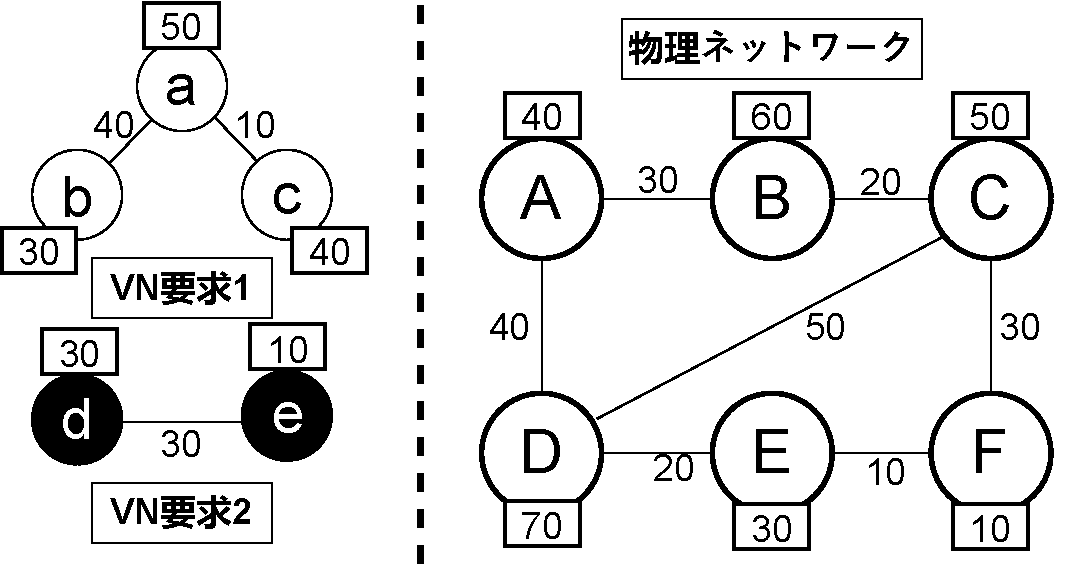
\includegraphics[width=8.0cm]{zu1.pdf}
  \caption{VN要求と物理ネットワークの例}
  \label{fig:network}
\end{figure}


\section{既存手法}

\noindent　当研究室では，2つの仮想ネットワーク埋め込み手法を
提案している\cite{second}\cite{third}．
両手法は，仮想ノードの埋め込みに貪欲法を用い，
仮想リンクの埋め込みにダイクストラ法を用いる．
貪欲法は，CPU需要が大きい仮想ノードから順に，
十分なCPU資源を持つ物理ノードへ埋め込む．
例えば，図1のVN要求1に貪欲法を適用すると，
仮想ノードの埋め込み優先順位はノードa，c，bとなる．
ダイクストラ法は，埋め込み先が決定した2つの仮想ノード間に
対応する物理ノード間の最短経路を求める．
その後，仮想リンクを最短経路を構成する物理リンクへ埋め込む．


\subsection{二ノ宮手法}

\noindent　二ノ宮は，物理リンクの残余帯域を参照して
仮想ノードの割当候補を決定する手法を提案した
\cite{second}．
本手法は，最初のVN要求に対して，
仮想ノードの埋め込みに貪欲法を用い，
仮想リンクの埋め込みにダイクストラ法を用いる．
2つ目以降のVN要求では，仮想リンクの帯域幅需要を満たす
物理リンクを抽出し，その物理リンクに接続する物理ノードを
仮想ノードの割当候補とする．
本手法は，候補の中からCPU資源が最大の物理ノードを選ぶ．
図\ref{fig:ninomiya}は，図\ref{fig:network}のネットワークに
二ノ宮手法を適用した結果を示す．
VN要求1を埋め込んだ後，VN要求2の帯域幅需要30を満たす
物理リンクを抽出すると，リンク$\{A，D\}$と$\{C，F\}$が
候補となる．本手法は，これらのリンクに接続する物理ノード
からVN要求2の割当先を決定する．
本手法は，帯域不足による仮想リンクの埋め込み失敗を抑える．
一方，仮想ノード数を$N_V$，物理ノード数を$N_S$とすると，
本手法の計算量は$\mathcal{O}(N_V N_S^3)$となる．

\begin{figure}[H]
  \centering
  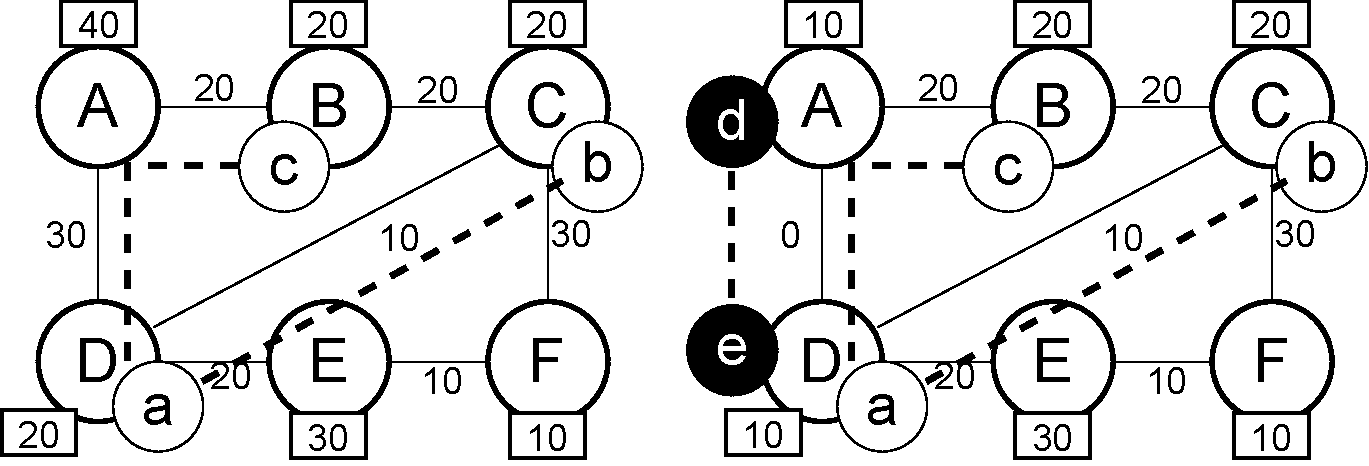
\includegraphics[width=8.0cm]{zu2and3.pdf}
  \caption{二ノ宮手法による埋め込み例}
  \label{fig:ninomiya}
\end{figure}

\subsection{寺生手法}
\noindent　寺生は，各ノードに接続するリンクの帯域幅合計を
評価値とする手法を提案した\cite{third}．
本手法は，接続する仮想リンクの帯域幅需要合計が大きい
仮想ノードから順に埋め込む．
帯域幅需要合計が等しい場合は，
CPU需要が大きい仮想ノードを優先する．
本手法は，CPU需要を満たす物理ノードの中から，
接続する物理リンクの残余帯域合計が最大の物理ノードを
割当先として選ぶ．
仮想ノードの割り当て後，
ダイクストラ法を用いて仮想リンクを埋め込む．
図\ref{fig:terabu}は，図\ref{fig:network}のネットワークに
寺生手法を適用した結果を示す．
VN要求1では，仮想ノード$a$，$b$，$c$の帯域幅需要合計が
それぞれ50，40，10となるため，
本手法は$a$，$b$，$c$の順に埋め込む．
仮想ノード$a$の割当候補では，
物理ノード$D$のリンク帯域幅合計が最大となるため，
本手法は仮想ノード$a$を物理ノード$D$へ割り当てる．
本手法は，帯域幅需要が大きい仮想ノードを，
周辺の帯域資源が大きい物理ノードへ優先して割り当てる．
仮想ノード数を$N_V$，物理ノード数を$N_S$とすると，
本手法の計算量は$\mathcal{O}(N_V N_S^2)$となる．
\begin{figure}[H]
  \centering
  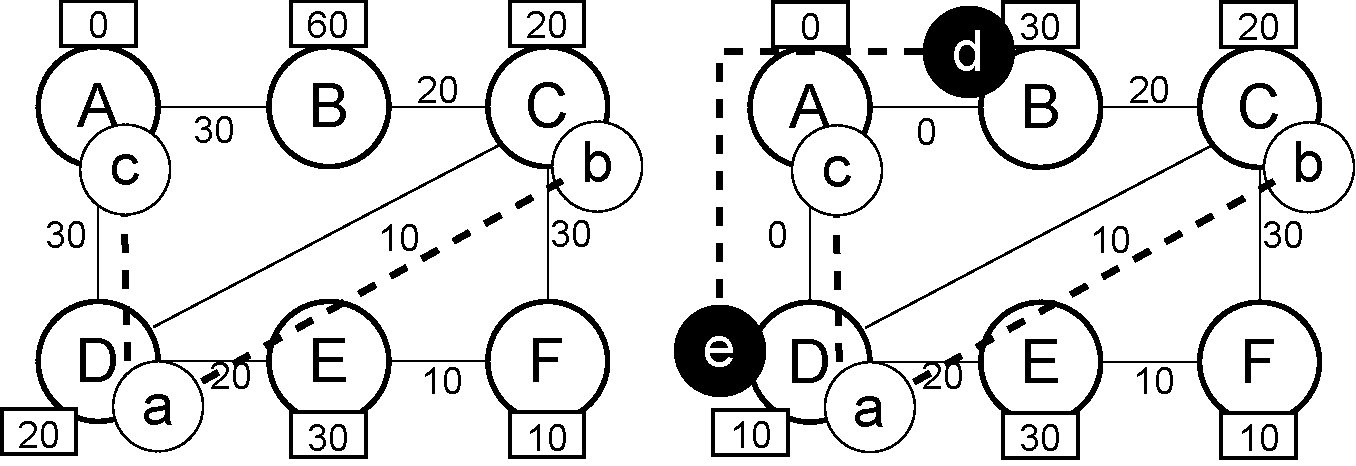
\includegraphics[width=8.0cm]{zu4and5.pdf}
  \caption{寺生手法による埋め込み例}
  \label{fig:terabu}
\end{figure}


\section{ALEVIN}

\noindent　ALEVIN（ALgorithms for Embedding VIrtual Networks）は，
VNEアルゴリズムの実装と性能評価を支援するシミュレータである．
ALEVINは，物理ネットワークと複数のVN要求を生成し，
各アルゴリズムによる埋め込み結果を評価する．
また，ALEVINはノードマッピングとリンクマッピングを
独立したクラスとして扱うため，
異なるノードマッピングとリンクマッピングを組み合わせられる．
本研究では，二ノ宮手法と寺生手法に基づく
ノードマッピングを実装した．
．
この実装により，リンクマッピングの条件を統一した上で，
二ノ宮手法と寺生手法のノード選択方法を比較できる．

\subsection{評価方法}  
\noindent　本研究では，VN要求の受理性能と物理資源の利用効率を
評価するため，AcceptedVnrRatio，CostRevenue，
AvPathLengthを用いる．

AcceptedVnrRatioは，全VN要求に対する
受理したVN要求の割合を表す．
受理したVN要求数を$N_{\mathrm{acc}}$，
全VN要求数を$N_{\mathrm{all}}$とすると，
AcceptedVnrRatioを次式で表す．
\[
 \mathrm{AcceptedVnrRatio}
 =
 \frac{N_{\mathrm{acc}}}{N_{\mathrm{all}}}
 \times 100
\]
AcceptedVnrRatioが大きいほど，
多くのVN要求を物理ネットワークへ埋め込める．

MappedRevenueは，受理したVN要求が持つ需要量を表す．
受理したVN要求に含まれる仮想ノードのCPU需要を
$d^{\mathrm{CPU}}_i$，
仮想リンクの帯域幅需要を$d^{\mathrm{BW}}_j$とすると，
MappedRevenueを次式で表す．
\[
 \mathrm{MappedRevenue}
 =
 \sum_i d^{\mathrm{CPU}}_i
 +
 \sum_j d^{\mathrm{BW}}_j
\]
Costは，VN要求の埋め込みによって
物理ネットワーク上で消費した資源量を表す．
物理ノードで消費したCPU資源を$c^{\mathrm{CPU}}_k$，
物理リンクで消費した帯域幅資源を
$c^{\mathrm{BW}}_l$とすると，Costを次式で表す．
\[
 \mathrm{Cost}
 =
 \sum_k c^{\mathrm{CPU}}_k
 +
 \sum_l c^{\mathrm{BW}}_l
\]
CostRevenueは，受理したVN要求の需要量に対する
物理資源の消費量を表す．
CostRevenueを次式で表す．
\[
 \mathrm{CostRevenue}
 =
 \frac{\mathrm{Cost}}
      {\mathrm{MappedRevenue}}
\]
CostRevenueが小さいほど，
少ない物理資源でVN要求を埋め込める．

AvPathLengthは，1本の仮想リンクが使用する
物理リンク数の平均値を表す．
AvPathLengthが小さいほど，
仮想リンクを短い経路へ埋め込める．


\section{比較実験}

\noindent　本実験では，寺生手法と二ノ宮手法の性能を比較する．
物理ネットワークのノード数を40または60とし，
各物理ネットワークに10個のVN要求を順に埋め込む．
物理ノードのCPU資源と物理リンクの帯域幅資源は，
それぞれ50以下の値として生成する．
物理ノード数が40の場合，各VN要求を4個の仮想ノードで
構成し，10個のVN要求に含まれる仮想ノードの総数を40とする．
物理ノード数が60の場合，各VN要求を6個の仮想ノードで
構成し，仮想ノードの総数を60とする．
VN要求には，表\ref{tab:demand-condition}に示す
3種類の需要条件を用いる．
以上から，物理ノード数と需要条件を組み合わせた
6種類のシナリオを用いる．

\begin{table}[H]
  \centering
  \caption{VN要求の需要条件}
  \label{tab:demand-condition}
  \begin{tabular}{c|c|c}
    \hline
    条件 & CPU需要 & 帯域幅需要 \\
    \hline
    1 & 25以下 & 25以下 \\
    2 & 25以下 & 10以下 \\
    3 & 10以下 & 25以下 \\
    \hline
  \end{tabular}
\end{table}

\section{実験結果}

\noindent　各実験条件について5回の実験を行い，
各評価指標の平均値を求めた．
表\ref{tab:result40}と表\ref{tab:result60}に実験結果を示す．
表中のC/RはCostRevenueを表し，
経路長はAvPathLengthを表す．

\begin{table}[H]
  \centering
  \caption{物理ノード数40の実験結果}
  \label{tab:result40}
  \footnotesize
  \setlength{\tabcolsep}{2.5pt}
  \renewcommand{\arraystretch}{1.1}
  \begin{tabular}{ccrrrr}
    \hline
    条件 & 手法 & 時間[s] & 受理率[\%] & C/R & 経路長 \\
    \hline
    1 & 寺生   & 0.819 & 94 & 1.000 & 1.000 \\
    1 & 二ノ宮 & 0.397 & 62 & 1.019 & 1.083 \\
    2 & 寺生   & 0.786 & 56 & 1.005 & 1.018 \\
    2 & 二ノ宮 & 0.356 & 78 & 1.025 & 1.050 \\
    3 & 寺生   & 0.491 & 72 & 1.020 & 1.050 \\
    3 & 二ノ宮 & 0.346 & 68 & 1.066 & 1.178 \\
    \hline
  \end{tabular}
\end{table}

\begin{table}[H]
  \centering
  \caption{物理ノード数60の実験結果}
  \label{tab:result60}
  \footnotesize
  \setlength{\tabcolsep}{2.5pt}
  \renewcommand{\arraystretch}{1.1}
  \begin{tabular}{ccrrrr}
    \hline
    条件 & 手法 & 時間[s] & 受理率[\%] & C/R & 経路長 \\
    \hline
    1 & 寺生   & 1.853 & 76 & 1.005 & 1.032 \\
    1 & 二ノ宮 & 0.780 & 50 & 1.008 & 1.043 \\
    2 & 寺生   & 1.889 & 30 & 1.008 & 1.042 \\
    2 & 二ノ宮 & 1.145 & 30 & 1.083 & 1.148 \\
    3 & 寺生   & 2.045 & 38 & 1.018 & 1.043 \\
    3 & 二ノ宮 & 1.099 & 28 & 1.039 & 1.067 \\
    \hline
  \end{tabular}
\end{table}

\noindent　寺生手法のAcceptedVnrRatioは，
6条件中4条件で二ノ宮手法を上回った．
条件2の物理ノード数60では，
両手法のAcceptedVnrRatioが30\%となった．
一方，条件2の物理ノード数40では，
二ノ宮手法が寺生手法を22\%上回った．

寺生手法のCostRevenueとAvPathLengthは，
すべての条件で二ノ宮手法以下となった．
一方，二ノ宮手法の実行時間は，
すべての条件で寺生手法より短くなった．

\section{考察}
\noindent　実験結果より，寺生手法は多くの条件で二ノ宮手法より高いAcceptedVnrRatioと低いCostRevenueを示した．
これは，リンク総容量に基づくノード選択が，短い埋め込み経路を実現し，後続要求の受理可能性を高めたためと考えられる．
一方で，実装上の実行時間は二ノ宮手法の方が短く，理論計算量との差異が見られた．この要因として，要求を早期に棄却してリンクマッピングの処理回数を減らした可能性がある．
今後はより大規模な条件で時間評価を行う必要がある．

\section{今後の課題}

\noindent　今後は，物理ネットワークの規模を変更し，
より多くのシナリオで両手法を比較する．
また，事前判定，ノードマッピング，リンクマッピングの
各処理時間と棄却数を記録し，
二ノ宮手法の実行時間が短くなった原因を明らかにする．

さらに，ALEVINにおけるネットワークの向きを検証する．
現在の実験では，物理ネットワークとVN要求を
有向グラフとして扱う場合と無向グラフとして扱う場合で，
経路探索や埋め込み結果が異なる可能性がある．
今後は，シナリオの生成処理，読み込み処理，
マッピング処理におけるグラフの向きを統一し，比較する．


\bibliographystyle{junsrt.bst}
\bibliography{citation.bib}


\end{document}
